\documentclass[a4paper]{article}

\usepackage{graphicx}
\usepackage{subfig}
\usepackage{multirow}
\usepackage[utf8]{inputenc}

\graphicspath{{figuras/}}

\hyphenation{ve-ri-fi-car FalaBrasil}

\title{Prova 2 - Sistemas de Controle Projetos}

\author{Pedro Batista (08080002701) - pedro@ufpa.br}

\begin{document}

\maketitle

\section{Projeto de Controlador PI ideal}\label{sec:pi_ideal}
Desejamos adicionar um controlador proporcional integral, no sistema
da Equação~\ref{eq:sis1} para levar a zero seu erro de regime, em
resposta ao degrau unitário. Como foi dado do problema o sistema
opera com coeficiente de amortecimento igual a $0.174$.

\begin{equation}
G(s)=\frac{1}{(s+1)(s+2)(s+10)}
\label{eq:sis1}
\end{equation}

Para levar o erro de regime a zero, adicionamos um polo em zero,
para que esse polo não influencie na resposta trasitória do sistema,
adicionamos também um zero próximo a este $-0.1$, o ganho $K$ também
é adicionado ao o sistema, e esse se torna
o mostrado na Equação~\ref{eq:sis1_pi}. Para este plotamos o LGR
e o coeficiente de amortecimento na Figura~\ref{fig:lgr_sis1},
podemos então definir o ganho do sistema. Simulamos
o sistema sem o controlador, e o sistema controlado na Figura~\ref{fig:sis1_sim}
onde podemos observar que o erro de regime será levado a zero.

\begin{equation}
G(s)=\frac{K(s+0.1)}{s(s+1)(s+2)(s+10)}
\label{eq:sis1_pi}
\end{equation}

\begin{figure}[ht]
   \centering
   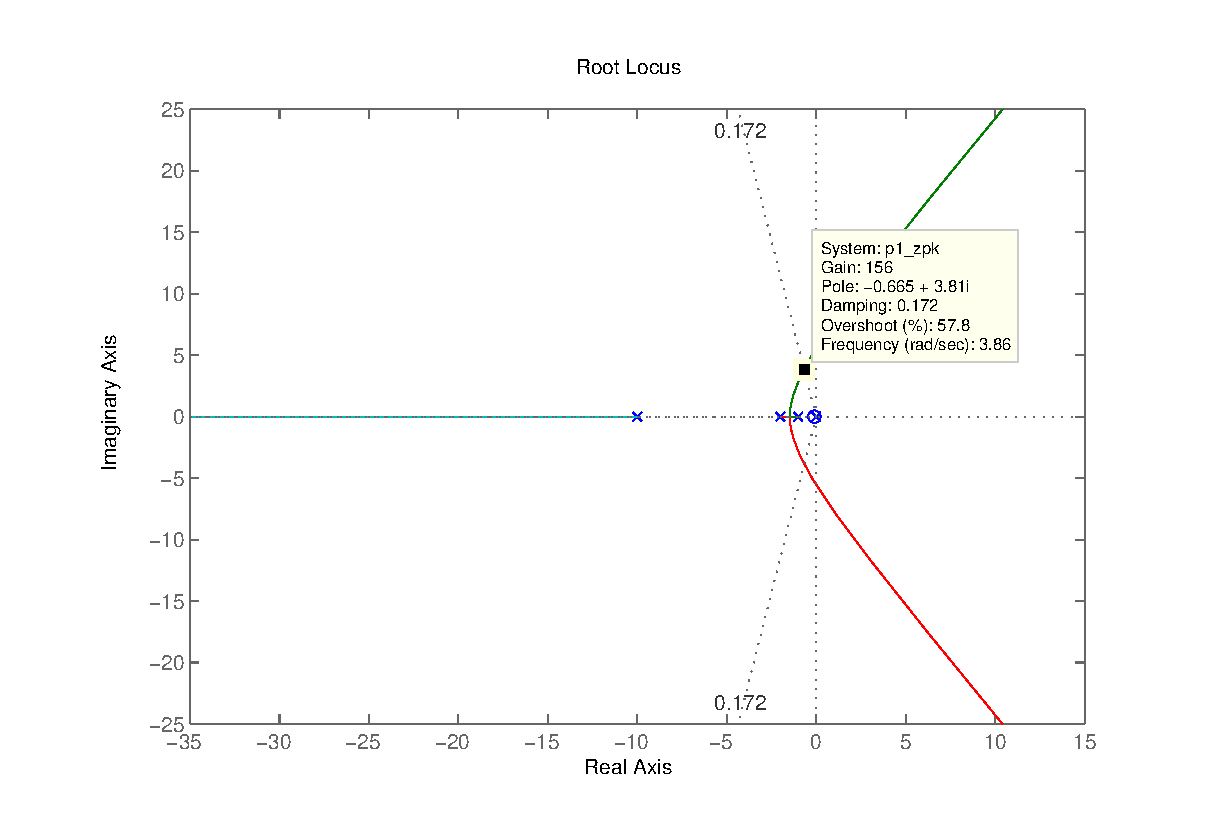
\includegraphics[width=0.9\textwidth]{p1_lgr}
   \caption{LGR para o sistema da Equação~\ref{eq:sis1}, com
      coeficiente de amortecimento igual a $0.174$.}
   \label{fig:lgr_sis1}
\end{figure}

\begin{figure}[ht]
   \centering
   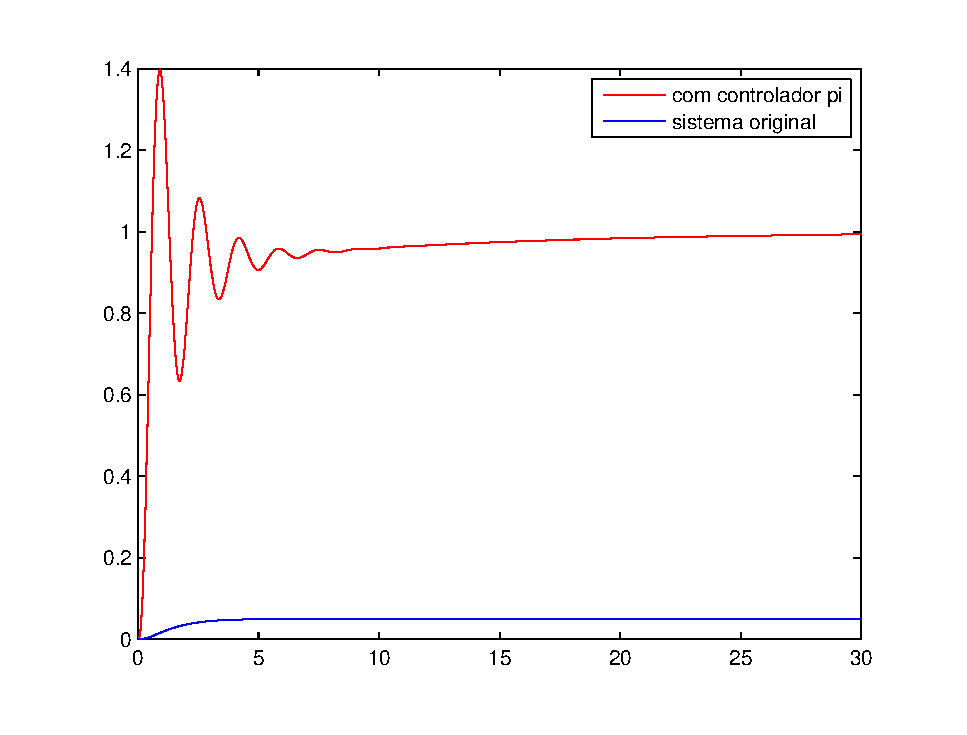
\includegraphics[width=0.9\textwidth]{p1_sim}
   \caption{Simulação para o sistema da Equação~\ref{eq:sis1},
      e sua versão controlada (Equação~\ref{eq:sis1_pi} com ganho
      $K=156$.}
   \label{fig:sis1_sim}
\end{figure}

Para gerar o LGR o código utilizado no matlab é mostrado na Figura~\ref{verb:sis1_lgr},
onde utilizamos o $zpk$ para representar o sistema, e o $rgrid$ para plotar o coeficiente
de amortecimento. Já para simulação dos sitemas usamos o esquema do $simulink$ mostrado
na Figura~\ref{fig:sis1_simulink}.

\begin{figure}[ht]
\begin{verbatim}
p1_zpk=zpk([-0.1], [0 -1 -2 -10], 1)
rlocus(p1_zpk)
sgrid(0.172, 'xi')
\end{verbatim}
\caption{Código do $MATLAB$ utilizado para plotar o LGR da Equação~\ref{eq:sis1_pi}}
\label{verb:sis1_lgr}
\end{figure}

\begin{figure}[ht]
   \subfloat[Esquema utilizado para o sistema não controlado (Equação~\ref{eq:sis1}).]
      {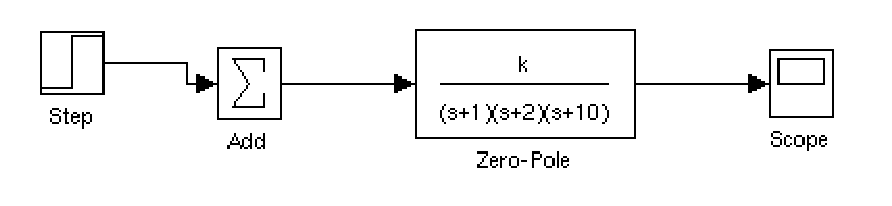
\includegraphics[width=0.5\textwidth]{sis1_simulink}}
   \subfloat[Esquema utilizado para o sistema controlado (Equação~\ref{eq:sis1_pi}).]
      {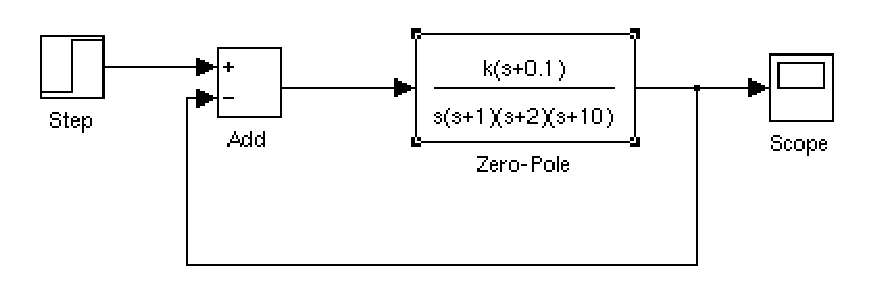
\includegraphics[width=0.5\textwidth]{sis1_simulink_pi}}
   \caption{Esquemas montados no $simulink$ para simular os sistemas
      do Problema~\ref{sec:pi_ideal}}
   \label{fig:sis1_simulink}
\end{figure}

\bibliographystyle{plain}
\bibliography{bib.bib} 
\end{document}
